% Provenance (never printed): see sources/outline_sources.md (Year 1: the wind-driven
% circulation, gyres, Ekman transport and upwelling, western boundary currents, the
% meridional overturning circulation and the water masses). Exercise and problem values in
% the Book 3 scratch calculator calc/ch29.py; figures from figdata/bachelor-1/
% ekman_hodograph.py (Ekman's solution with Ekman's constants) and stommel_gyre.py
% (Stommel's 1948 model, exercise parameters), the world map from figdata/shared/geo.py.
% Physics owns the Coriolis force (recalled). Book 1 (g8) gave the surface currents and
% the gyres in words, Book 2 (g10) upwelling: re-founded here with the Ekman balance.
% Ch. 26 owns the T-S diagram and the water masses, ch. 28 the Coriolis parameter, the
% geostrophic wind and the mean meridional streamfunction. The Sverdrup balance, the
% vorticity argument and the derivation of the Ekman spiral are the Year 3 volume's; ENSO
% the Year 2 volume's.
\chapter{The Circulation of the Ocean}\label{ch:b1:ocean-circulation}

In 1992, during a storm in the North Pacific, a container washed overboard from a
ship sailing from Hong Kong to the United States. It broke open and released about
\num{29000} rubber ducks and other bath toys, which floated away and travelled far
and wide; the places where some of them were later found helped scientists to
understand the currents that had carried them. Floating toys
follow the surface water, and the surface water of the oceans does not wander at
random: it turns in basin-wide \omterm{def:b1:ocean-circulation:gyre}{gyres}, races north in narrow currents along the
western coasts of the oceans, and rises or sinks in a few chosen places. This
chapter explains how the wind sets the upper ocean moving, why the water moves at
right angles to the wind that pushes it, why the strongest currents hug the western
sides of the oceans, and how a slow overturning carries water to the abyss and back.
% ledger: noaa:floatees

\begin{omfigure}
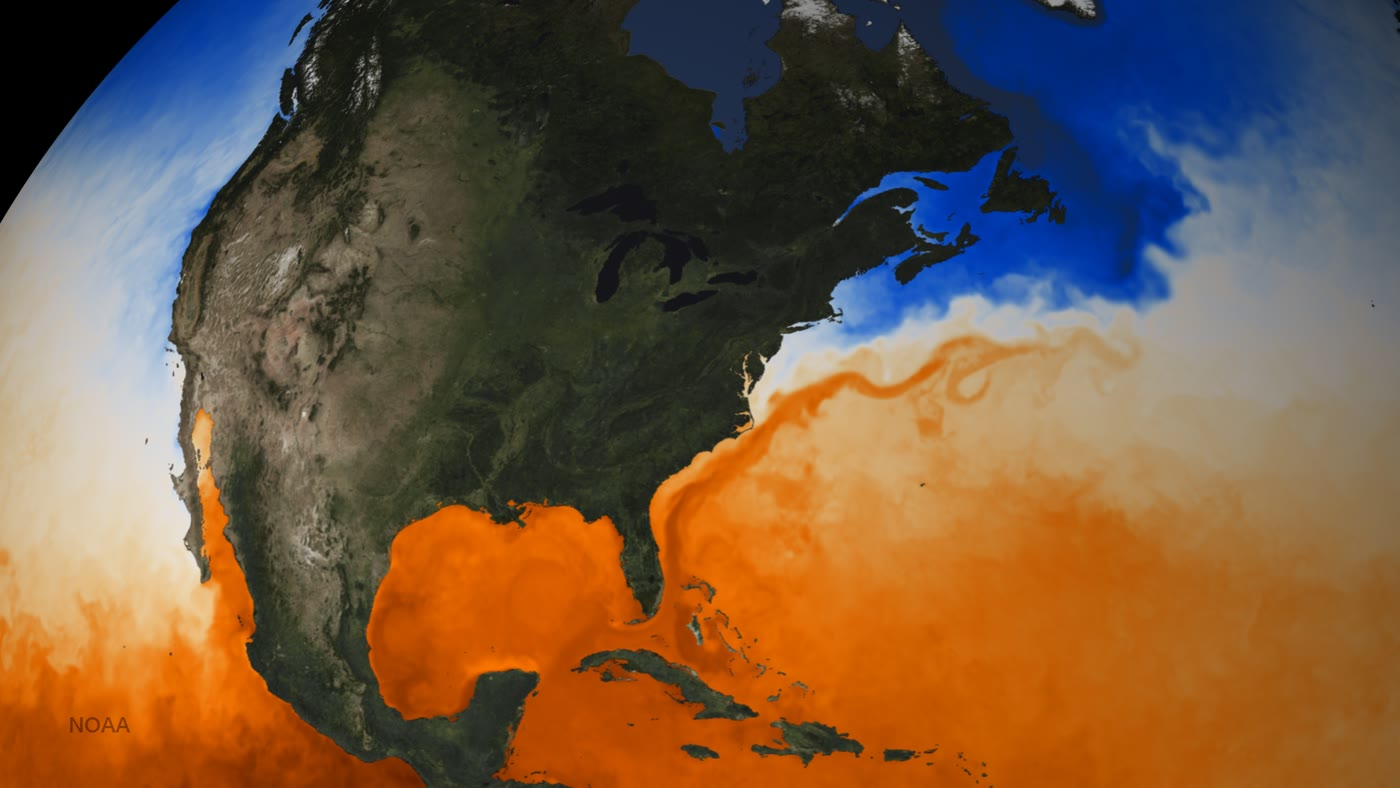
\includegraphics[width=0.85\linewidth]{images/book3/b1-gulf-stream-sst.jpg}

{\small The temperature of the sea surface around North America in early June 2016,
from satellite data (warm water in orange, cold water in blue). The Gulf Stream
leaves the coast of the United States as a warm, meandering ribbon and crosses the
Atlantic towards Europe; at the same \omterm{def:b1:spherical-astronomy:geographic}{latitudes}, the water off the Pacific coast is
much cooler than off the Atlantic coast. (NOAA, NESDIS, public domain, via
Wikimedia Commons.)}
\label{fig:b1:ocean-circulation:sst}
\end{omfigure}
% ledger: commons:gulf-stream-sst, noaa:gulf-stream-heat

\begin{recall}
The physics volumes give the Coriolis force. \Cref{ch:b1:atmospheric-circulation}
wrote its horizontal part as $-f\,\vec k\times\vec v$, with the \omterm{def:b1:atmospheric-circulation:coriolis-parameter}{Coriolis parameter}
$f = 2\Omega\sin\varphi$ ($\Omega = \qty{7.292e-5}{rad.s^{-1}}$), and found the
\omterm{def:b1:atmospheric-circulation:winds}{trade winds}, easterlies between the equator and about \ang{30}, and the \omterm{def:b1:atmospheric-circulation:winds}{westerlies}
beyond; it also defined the \omterm{def:b1:atmospheric-circulation:streamfunction}{mean meridional streamfunction} of an overturning.
\Cref{ch:b1:fluid-envelopes-structure} gave the \omterm{def:b1:fluid-envelopes-structure:ocean-layers}{mixed layer} and the \omterm{def:b1:fluid-envelopes-structure:ocean-layers}{thermocline}, the
density of seawater, the \omterm{def:b1:fluid-envelopes-structure:ts-diagram}{T--S diagram} and the water masses of the South Atlantic,
and \cref{ch:b1:radiation-heat-transport} the poleward heat transport shared by the
atmosphere and the ocean. Book~1 described the surface currents and the great
\omterm{def:b1:ocean-circulation:gyre}{gyres}; Book~2 the \omterm{def:b1:ocean-circulation:upwelling}{upwelling} of cold water along some coasts.
% ledger: earth:Trot, nos:gyres
\end{recall}

\section{The wind and the surface currents}\label{sec:b1:ocean-circulation:wind}

The wind moves the sea by rubbing on it. Its force is spread over the surface, and
it is measured, like a pressure, per unit area.

\begin{definition}[Wind stress]\label{def:b1:ocean-circulation:wind-stress}
The \emph{wind stress}\index{wind stress} $\vec T$ is the horizontal force per unit
area exerted by the wind on the sea surface, in pascals. It is the downward transfer
of the horizontal momentum of the air into the ocean, and points nearly along the
wind. Its size is given by the bulk formula
\[
  T = \rho_a C_D U_{10}^2,
\]
where $\rho_a = \qty{1.3}{kg.m^{-3}}$ is the density of air, $U_{10}$ the wind speed
\qty{10}{m} above the sea and $C_D$ a dimensionless drag coefficient.
\end{definition}
% ledger: stewart:wind-stress

The drag coefficient is measured with fast instruments that record the turbulent
fluctuations of the wind a few metres above the waves. For a neutrally stable air,
the measurements of Yelland and Taylor give
\[
  1000\,C_D = 0.29 + \frac{3.1}{U_{10}} + \frac{7.7}{U_{10}^2}
  \quad (\qtyrange{3}{6}{m/s}),
  \qquad
  1000\,C_D = 0.60 + 0.071\,U_{10}
  \quad (\qtyrange{6}{26}{m/s}),
\]
with $U_{10}$ in metres per second. A wind of \qty{10}{m/s} has $C_D =
\num{1.31e-3}$ and exerts $T = 1.3 \times \num{1.31e-3} \times 100 =
\qty{0.170}{Pa}$; a wind of \qty{5}{m/s}, \qty{0.040}{Pa}; a gale of
\qty{20}{m/s}, \qty{1.05}{Pa}. Doubling the wind from 10 to \qty{20}{m/s}
multiplies the stress by $6.2$, not by $4$: rougher seas grip the wind harder. These
stresses are minute, a millionth of the atmospheric pressure, but they act without
pause on the whole ocean.
% ledger: stewart:drag-coefficient (computed in figdata/bachelor-1/ekman_hodograph.py and calc/ch29.py)

The pattern of the stress follows that of the winds. Between the \omterm{def:b1:atmospheric-circulation:winds}{trade winds} of the
tropics, blowing towards the west, and the \omterm{def:b1:atmospheric-circulation:winds}{westerlies} of the \omterm{def:b1:spherical-astronomy:geographic}{mid-latitudes}, blowing
towards the east, the surface water of each ocean basin is set turning.

\begin{definition}[Gyre; subtropical and subpolar gyres]\label{def:b1:ocean-circulation:gyre}
A \emph{gyre}\index{gyre} is a large system of rotating ocean currents filling an
ocean basin. A \emph{subtropical gyre}\index{subtropical gyre} lies between the \omterm{def:b1:atmospheric-circulation:winds}{trade
winds} and the \omterm{def:b1:atmospheric-circulation:winds}{westerlies} and turns clockwise in the Northern Hemisphere and
anticlockwise in the Southern. A \emph{subpolar gyre}\index{subpolar gyre} lies on
the poleward side of the \omterm{def:b1:atmospheric-circulation:winds}{westerlies} and turns the other way.
\end{definition}
% ledger: nos:gyre-def, nos:boundary-currents, stewart:north-atlantic

There are five \omterm{def:b1:ocean-circulation:gyre}{subtropical gyres}, in the North and South Atlantic, the North and
South Pacific and the Indian Ocean; none straddles the equator. In the North
Atlantic, the \omterm{def:b1:ocean-circulation:gyre}{subtropical gyre} is closed by the Gulf Stream along the coast of the
United States in the west and by the Canary Current off Africa in the east; north
of it, the \omterm{def:b1:ocean-circulation:gyre}{subpolar gyre} turns anticlockwise, with the North Atlantic Current on its
southern side and the Labrador Current flowing south along its western side. At low
\omterm{def:b1:spherical-astronomy:geographic}{latitudes}, the westward equatorial currents of the Atlantic and the Pacific are
separated by an eastward countercurrent. The \omterm{def:b1:ocean-circulation:gyre}{gyres} are not symmetric: every \omterm{def:b1:ocean-circulation:gyre}{subtropical gyre} is
closed by a strong, narrow current on the western side of its basin and by a weak,
broad current on the eastern side. Around Antarctica, where no continent stops it,
the Antarctic Circumpolar Current flows eastward round the globe, driven by the
\omterm{def:b1:atmospheric-circulation:winds}{westerlies} of the Southern Ocean.
% ledger: nos:boundary-currents, stewart:north-atlantic, stewart:heat-conveyor, lien:kuroshio, donohue:acc, stewart:acc

\begin{omfigure}
\begin{tikzpicture}
\begin{axis}[ommap, width=0.98\linewidth, xtick={-180,-120,...,180}, ytick={-60,-30,0,30,60}]
% land: figdata/shared/geo.py; ledger: data:ne-land. Arrows placed by hand from the
% ledgered pattern: nos:boundary-currents, stewart:north-atlantic, lien:kuroshio,
% donohue:acc, stewart:acc
\addplot[fill=omLithAlluv, draw=black!45, line width=0.2pt, forget plot] table {figdata/out/shared-geo-land.dat};
% North Atlantic subtropical gyre (clockwise)
\addplot[omThm, line width=1.1pt, -{Stealth[length=4pt]}, smooth] coordinates {(-80,26) (-77,32) (-70,37) (-58,40) (-44,41)};
\addplot[omThm, line width=1.1pt, -{Stealth[length=4pt]}, smooth] coordinates {(-38,40) (-28,39) (-20,36)};
\addplot[omThm, line width=1.1pt, -{Stealth[length=4pt]}, smooth] coordinates {(-19,32) (-21,24) (-26,17)};
\addplot[omThm, line width=1.1pt, -{Stealth[length=4pt]}, smooth] coordinates {(-32,14) (-45,13) (-60,15)};
% North Atlantic subpolar gyre (anticlockwise)
\addplot[omDef, line width=1.1pt, -{Stealth[length=4pt]}, smooth] coordinates {(-40,47) (-28,52) (-18,57)};
\addplot[omDef, line width=1.1pt, -{Stealth[length=4pt]}, smooth] coordinates {(-24,61) (-35,62) (-44,59)};
\addplot[omDef, line width=1.1pt, -{Stealth[length=4pt]}, smooth] coordinates {(-55,59) (-56,53) (-51,47)};
% North Pacific subtropical gyre (clockwise)
\addplot[omThm, line width=1.1pt, -{Stealth[length=4pt]}, smooth] coordinates {(123,19) (125,26) (133,32) (143,36) (156,38)};
\addplot[omThm, line width=1.1pt, smooth] coordinates {(162,39) (172,40) (180,40.5)};
\addplot[omThm, line width=1.1pt, -{Stealth[length=4pt]}, smooth] coordinates {(-180,40.5) (-165,41) (-148,40)};
\addplot[omThm, line width=1.1pt, -{Stealth[length=4pt]}, smooth] coordinates {(-133,37) (-128,29) (-122,20)};
\addplot[omThm, line width=1.1pt, -{Stealth[length=4pt]}, smooth] coordinates {(-125,13) (-150,12) (-175,13)};
\addplot[omThm, line width=1.1pt, -{Stealth[length=4pt]}, smooth] coordinates {(170,13) (152,14) (135,15)};
% South Atlantic subtropical gyre (anticlockwise)
\addplot[omThm, line width=1.1pt, -{Stealth[length=4pt]}, smooth] coordinates {(2,-8) (-15,-9) (-30,-9)};
\addplot[omThm, line width=1.1pt, -{Stealth[length=4pt]}, smooth] coordinates {(-34,-14) (-39,-24) (-47,-34)};
\addplot[omThm, line width=1.1pt, -{Stealth[length=4pt]}, smooth] coordinates {(-42,-40) (-20,-40) (2,-38)};
\addplot[omThm, line width=1.1pt, -{Stealth[length=4pt]}, smooth] coordinates {(10,-31) (9,-23) (6,-15)};
% South Pacific subtropical gyre (anticlockwise)
\addplot[omThm, line width=1.1pt, -{Stealth[length=4pt]}, smooth] coordinates {(-88,-10) (-120,-11) (-160,-12)};
\addplot[omThm, line width=1.1pt, -{Stealth[length=4pt]}, smooth] coordinates {(160,-16) (157,-26) (162,-35)};
\addplot[omThm, line width=1.1pt, -{Stealth[length=4pt]}, smooth] coordinates {(-170,-40) (-140,-41) (-105,-39)};
\addplot[omThm, line width=1.1pt, -{Stealth[length=4pt]}, smooth] coordinates {(-82,-36) (-82,-27) (-85,-17)};
% Indian Ocean subtropical gyre (anticlockwise)
\addplot[omThm, line width=1.1pt, -{Stealth[length=4pt]}, smooth] coordinates {(98,-13) (80,-14) (60,-15)};
\addplot[omThm, line width=1.1pt, -{Stealth[length=4pt]}, smooth] coordinates {(47,-22) (40,-29) (33,-34)};
\addplot[omThm, line width=1.1pt, -{Stealth[length=4pt]}, smooth] coordinates {(50,-38) (75,-37) (100,-35)};
\addplot[omThm, line width=1.1pt, -{Stealth[length=4pt]}, smooth] coordinates {(108,-31) (106,-24) (102,-18)};
% Antarctic Circumpolar Current (eastward)
\addplot[omMeth, line width=1.4pt, -{Stealth[length=5pt]}, smooth] coordinates {(-62,-58) (-40,-55) (-15,-52)};
\addplot[omMeth, line width=1.4pt, -{Stealth[length=5pt]}, smooth] coordinates {(5,-52) (40,-50) (75,-50)};
\addplot[omMeth, line width=1.4pt, -{Stealth[length=5pt]}, smooth] coordinates {(95,-51) (130,-53) (165,-56)};
\addplot[omMeth, line width=1.4pt, -{Stealth[length=5pt]}, smooth] coordinates {(-170,-58) (-130,-59) (-85,-59)};
\node[font=\scriptsize, anchor=west, fill=white, fill opacity=0.8, text opacity=1, inner sep=1pt] at (axis cs:-66,31) {Gulf Stream};
\node[font=\scriptsize, anchor=west, fill=white, fill opacity=0.8, text opacity=1, inner sep=1pt] at (axis cs:-11,25) {Canary};
\node[font=\scriptsize, anchor=east, fill=white, fill opacity=0.8, text opacity=1, inner sep=1pt] at (axis cs:-58,52) {Labrador};
\node[font=\scriptsize, anchor=west, fill=white, fill opacity=0.8, text opacity=1, inner sep=1pt] at (axis cs:142,28) {Kuroshio};
\node[font=\scriptsize, anchor=north, fill=white, fill opacity=0.8, text opacity=1, inner sep=1pt] at (axis cs:-150,9) {North Equatorial};
\node[font=\scriptsize, anchor=north, fill=white, fill opacity=0.8, text opacity=1, inner sep=1pt] at (axis cs:0,-62) {Antarctic Circumpolar Current};
\end{axis}
\end{tikzpicture}

{\small The \omterm{def:b1:ocean-circulation:gyre}{gyres} of the surface ocean (schematic arrows on a map of the land).
Dark red: the five \omterm{def:b1:ocean-circulation:gyre}{subtropical gyres}, clockwise in the Northern Hemisphere and
anticlockwise in the Southern, each with a narrow \omterm{def:b1:ocean-circulation:wbc}{western boundary current}; blue:
the \omterm{def:b1:ocean-circulation:gyre}{subpolar gyre} of the North Atlantic; green: the Antarctic Circumpolar Current.
Named are only the currents discussed in the text. The arrows show the sense of the
flow, not its speed.}
\label{fig:b1:ocean-circulation:gyres}
\end{omfigure}
% ledger: data:ne-land, nos:boundary-currents, stewart:north-atlantic, lien:kuroshio, donohue:acc

Two features of this pattern need explaining. The first is the sense of rotation:
the \omterm{def:b1:atmospheric-circulation:winds}{trade winds} blow towards the west on the equatorward side of a \omterm{def:b1:ocean-circulation:gyre}{subtropical gyre},
yet the currents of the \omterm{def:b1:ocean-circulation:gyre}{gyre} do not simply follow the winds, and the surface water
drifts at an angle to them. The second is the asymmetry: the return flow of a \omterm{def:b1:ocean-circulation:gyre}{gyre}
is crushed against the western side of its basin. Both come from the rotation of
the Earth.

\section{Ekman transport}\label{sec:b1:ocean-circulation:ekman}

\begin{history}[Nansen and Ekman, 1898--1905]
During his expedition in the Arctic, Fridtjof Nansen noticed that the wind drove
the sea ice not along the wind but at an angle of \ang{20} to \ang{40} to its
right, looking downwind. He reasoned that three forces had to balance on the moving
ice: the push of the wind, the friction of the water, and the Coriolis force. He
asked the meteorologist Vilhelm Bjerknes to let one of his students study the
influence of the Earth's rotation on wind-driven currents. The student, Walfrid
Ekman, worked out the theory for his doctoral thesis at Uppsala, and extended it in
1905. His solution is still the starting point of the theory of the wind-driven
ocean.
\end{history}
% ledger: stewart:ekman-layer, nos:ekman-spiral

\begin{definition}[Ekman layer, Ekman transport, Ekman spiral]\label{def:b1:ocean-circulation:ekman}
The \emph{Ekman layer}\index{Ekman layer} is the thin surface layer of the ocean,
at most a few hundred metres thick, in which the stress of the wind is carried down
by turbulent friction and balanced by the Coriolis force. The \emph{Ekman
transport}\index{Ekman transport} is the mass of water that the layer carries per
second across a vertical strip \qty{1}{m} wide, from the surface down to below the
layer:
\[
  \vec M = \int_{-d}^{0} \rho\,\vec v\,\mathrm dz \quad (\unit{kg.m^{-1}.s^{-1}});
\]
divided by the density, it is a volume transport per metre, in
\unit{m^2.s^{-1}}. The \emph{Ekman spiral}\index{Ekman spiral} is the turning and
weakening of the current with depth in the layer. Ocean transports are counted in
\emph{sverdrups}\index{sverdrup (unit)}: \qty{1}{\sverdrup} $=
\qty{e6}{m^3.s^{-1}}$.
\end{definition}
% ledger: stewart:ekman-layer, stewart:ekman-transport

\begin{theorem}[Ekman transport]\label{thm:b1:ocean-circulation:ekman}
In a steady state, far from coasts, over water much deeper than the \omterm{def:b1:ocean-circulation:ekman}{Ekman layer}, the
\omterm{def:b1:ocean-circulation:ekman}{Ekman transport} depends only on the \omterm{def:b1:ocean-circulation:wind-stress}{wind stress} $\vec T$ and on the \omterm{def:b1:atmospheric-circulation:coriolis-parameter}{Coriolis
parameter} $f$:
\[
  \vec M = \frac{1}{f}\,\vec T\times\vec k,
  \qquad |\vec M| = \frac{|\vec T|}{|f|}.
\]
It is at right angles to the \omterm{def:b1:ocean-circulation:wind-stress}{wind stress}, to its right in the Northern Hemisphere
and to its left in the Southern.
\end{theorem}
% ledger: stewart:ekman-transport

\begin{proof}
Let $\vec\tau(z)$ be the horizontal stress that the water above the level $z$
exerts on the water below it. At the surface it is the \omterm{def:b1:ocean-circulation:wind-stress}{wind stress}, $\vec\tau(0) =
\vec T$; below the layer, where the currents driven by the wind have died away, it
vanishes, $\vec\tau(-d) = \vec 0$. A thin slab between $z$ and $z + \mathrm dz$, of
unit horizontal area, receives $\vec\tau(z + \mathrm dz)$ on its top face and
$-\vec\tau(z)$ on its bottom face: the net friction force is $(\partial\vec
\tau/\partial z)\,\mathrm dz$. Its mass is $\rho\,\mathrm dz$, and the horizontal
Coriolis force on it is $-f\,\vec k\times\vec v\,\rho\,\mathrm dz$. In a steady
state, with no horizontal change from place to place, the two balance:
\[
  -f\rho\,\vec k\times\vec v + \frac{\partial\vec\tau}{\partial z} = \vec 0 .
\]
Integrating from $-d$ to $0$,
\[
  -f\,\vec k\times\vec M + \vec\tau(0) - \vec\tau(-d) = \vec 0,
  \qquad\text{that is}\qquad \vec k\times\vec M = \frac{\vec T}{f}.
\]
For a horizontal vector, $\vec k\times(\vec k\times\vec M) = -\vec M$; taking
$\vec k\times$ of both sides gives $-\vec M = \vec k\times\vec T/f$, so $\vec M =
\vec T\times\vec k/f$. The vector $\vec T\times\vec k$ is $\vec T$ turned by
\ang{90} clockwise seen from above: to the right of the wind when $f > 0$, to the
left when $f < 0$. Its size is $|\vec T|$.
\end{proof}

The result does not depend on how the friction works inside the layer, which is
poorly known: only the stress at the top and its vanishing at the bottom enter.
This makes the transport far more robust than the velocities themselves. The water
of the whole layer, taken together, moves at right angles to the wind, a result that
seems strange until one remembers that over a day or more the Coriolis force has
time to turn every current.

\begin{example}[The transport under a fresh breeze]\label{ex:b1:ocean-circulation:transport}
A wind of \qty{10}{m/s} blowing towards the north at \ang{35} N exerts
$T = \qty{0.170}{Pa}$. With $f = 2\Omega\sin\ang{35} = \qty{8.365e-5}{s^{-1}}$, the
\omterm{def:b1:ocean-circulation:ekman}{Ekman transport} is $0.170/(\num{8.365e-5}) = \qty{2036}{kg.m^{-1}.s^{-1}}$, towards
the east. With $\rho = \qty{1027}{kg.m^{-3}}$, this is \qty{1.98}{m^3.s^{-1}} for
each metre measured across the transport: across a line \qty{1000}{km} long, about
\qty{2}{\sverdrup}.
\end{example}
% ledger: stewart:drag-coefficient, stewart:ekman-constants, earth:Trot (computed in calc/ch29.py)

The theorem has been tested at sea. Across \ang{11} N in the Atlantic, where the
\omterm{def:b1:atmospheric-circulation:winds}{trade winds} blow towards the west, the \omterm{def:b1:ocean-circulation:ekman}{Ekman transport} is northward; measured
directly with a current profiler, it came to
\qty[uncertainty-mode=separate]{12.0 \pm 5.5}{\sverdrup}, against
\qty[uncertainty-mode=separate]{8.8 \pm 1.9}{\sverdrup} computed from the winds
measured during the survey and
\qty[uncertainty-mode=separate]{13.5 \pm 0.3}{\sverdrup} from winds averaged over
many years.
% ledger: stewart:ekman-transport

How the current is distributed with depth inside the layer depends on the
friction. Ekman took the simplest model, a turbulent friction proportional to the
vertical shear of the current, $\vec\tau = \rho A_z\,\partial\vec v/\partial z$, with
a constant eddy viscosity $A_z$.

\begin{proposition}[The Ekman spiral]\label{prop:b1:ocean-circulation:spiral}
For a steady \omterm{def:b1:ocean-circulation:wind-stress}{wind stress} $T$ towards the north over a deep, homogeneous ocean in the
Northern Hemisphere, with a constant eddy viscosity $A_z$, the current at height $z
\leq 0$ is
\[
  u = V_0\,e^{az}\cos\Bigl(\frac\pi4 + az\Bigr),\qquad
  v = V_0\,e^{az}\sin\Bigl(\frac\pi4 + az\Bigr),\qquad
  a = \sqrt{\frac{f}{2A_z}},\quad V_0 = \frac{T}{\rho\sqrt{fA_z}},
\]
with $u$ eastward and $v$ northward. At the surface the current flows at \ang{45} to
the right of the wind; with depth it weakens as $e^{az}$ and turns further to the
right. At the depth $D_E = \pi/a$, the Ekman depth, it flows against the surface
current with $e^{-\pi} = \num{0.043}$ of its speed.
\end{proposition}
\admitted
% ledger: stewart:ekman-solution

The derivation solves the two equations $f v + A_z u'' = 0$ and $-f u + A_z v'' =
0$ of the balance in the proof above; it is done in the Year~3 volume, and
\cref{exo:b1:ocean-circulation:10} checks that the formulas satisfy the equations
and that the spiral carries exactly the transport of the theorem. To use the
spiral, one needs $A_z$, which is not measured directly. Ekman gathered the
observed speeds of surface currents and found, for $|\varphi| \geq \ang{10}$,
\[
  V_0 = \frac{0.0127\,U_{10}}{\sqrt{\sin|\varphi|}},
  \qquad\text{which gives}\qquad
  D_E = \frac{7.6\,U_{10}}{\sqrt{\sin|\varphi|}},
\]
in SI units, with his drag coefficient $C_D = \num{2.6e-3}$ and $\rho_a =
\qty{1.25}{kg.m^{-3}}$. At \ang{35} N under a wind of \qty{10}{m/s}, $D_E =
\qty{100}{m}$ and $V_0 = \qty{0.17}{m/s}$; the \omterm{def:b1:ocean-circulation:ekman}{Ekman layer} ranges from about
\qty{45}{m} under light winds at \omterm{def:b1:spherical-astronomy:geographic}{mid-latitudes} to \qty{300}{m} under a gale in the
tropics, and the surface current is \qtyrange{1}{2.5}{\percent} of the wind.
% ledger: stewart:ekman-constants (computed in figdata/bachelor-1/ekman_hodograph.py)

\begin{omfigure}
\begin{tikzpicture}
\begin{axis}[ompt, name=hodo, width=0.5\linewidth, axis equal image, xmin=-6, xmax=22,
  ymin=-6, ymax=17, xlabel={eastward current (\unit{cm/s})}, ylabel={northward current (\unit{cm/s})},
  xtick={-5,0,5,10,15,20}, ytick={-5,0,5,10,15}]
% figdata/bachelor-1/ekman_hodograph.py; ledger: stewart:ekman-solution, stewart:ekman-constants
\addplot[black!45, line width=0.6pt] table[x expr=\thisrow{u}*100, y expr=\thisrow{v}*100] {figdata/out/bachelor-1-ekman_hodograph-tips.dat};
\addplot[omDef, line width=0.6pt, -{Stealth[length=3pt]}, quiver={u=\thisrow{u}*100, v=\thisrow{v}*100}]
  table[x expr=0, y expr=0] {figdata/out/bachelor-1-ekman_hodograph-arrows.dat};
\draw[omThm, line width=1.6pt, -{Stealth[length=6pt]}] (axis cs:-3,0) -- (axis cs:-3,14);
\node[font=\scriptsize, text=omThm, anchor=west] at (axis cs:-2.6,13) {wind};
\draw[omMeth, line width=1.6pt, -{Stealth[length=6pt]}] (axis cs:0,-3.2) -- (axis cs:16,-3.2);
\node[font=\scriptsize, text=omMeth, anchor=north] at (axis cs:8,-3.6) {Ekman transport};
\node[font=\scriptsize, anchor=south west] at (axis cs:11.9,11.9) {surface};
\node[font=\scriptsize, anchor=north east] at (axis cs:-0.3,-0.4) {$D_E$};
\end{axis}
\begin{axis}[ompt, at={(hodo.east)}, anchor=west, xshift=1.4cm, width=0.42\linewidth, height=6.2cm,
  xmin=-4, xmax=14, ymin=-200, ymax=0, xlabel={current (\unit{cm/s})}, ylabel={depth (\unit{m})},
  yticklabel={$\pgfmathprintnumber[fixed]{\tick}$},
  legend style={font=\scriptsize, at={(0.97,0.03)}, anchor=south east, cells={anchor=west}}]
\addplot[black!40, forget plot] coordinates {(0,-200) (0,0)};
\addplot[omDef, line width=1pt] table[x expr=\thisrow{u}*100, y=z] {figdata/out/bachelor-1-ekman_hodograph-profile.dat};
\addlegendentry{eastward}
\addplot[omProp, line width=1pt, dashed] table[x expr=\thisrow{v}*100, y=z] {figdata/out/bachelor-1-ekman_hodograph-profile.dat};
\addlegendentry{northward}
\addplot[black!50, densely dotted, forget plot] coordinates {(-4,-100.35) (14,-100.35)};
\node[font=\scriptsize, anchor=south east] at (axis cs:13.8,-100.35) {$D_E = \qty{100}{m}$};
\end{axis}
\end{tikzpicture}

{\small Ekman's spiral under a wind of \qty{10}{m/s} blowing towards the north at
\ang{35} N, with Ekman's constants. Left: the current seen from above at the
surface and every tenth of the Ekman depth $D_E$ down to $D_E$ (blue arrows), the
grey curve joining their tips; the surface current is \ang{45} to the right of the
wind, the deeper ones are weaker and turned further right. The transport of the
whole layer (green; direction only) is at \ang{90} to the right of the wind.
Right: the two components against depth.}
\label{fig:b1:ocean-circulation:spiral}
\end{omfigure}
% ledger: stewart:ekman-solution, stewart:ekman-constants

The spiral is an idealisation. Measurements from current meters on moorings and
from 1503 drifters followed in the Pacific between 1987 and 1994 show that, averaged
over many days, the flow agrees remarkably well with Ekman's theory: the depth of the
layer is almost his, $7.12\,U_{10}/\sqrt{\sin|\varphi|}$; the surface current is
about half his value; the angle between the wind and the surface flow is near
\ang{45} at \omterm{def:b1:spherical-astronomy:geographic}{mid-latitudes}; and the transport is at \ang{90} to the right of the wind.
Over a few hours, the picture is blurred by inertial oscillations, and the balance
needs the wind to blow steadily for a day or two to establish itself.
% ledger: stewart:ekman-observed

\section{Upwelling and Ekman pumping}\label{sec:b1:ocean-circulation:upwelling}

Where the \omterm{def:b1:ocean-circulation:ekman}{Ekman transport} is not the same everywhere, water piles up in some places
and is drawn away from others; the difference is made up by vertical motion.

\begin{definition}[Upwelling, downwelling, coastal upwelling]\label{def:b1:ocean-circulation:upwelling}
\emph{Upwelling}\index{upwelling} is the rise of water from below into the surface
layer of the ocean, to replace surface water carried away; \emph{downwelling}%
\index{downwelling} is the sinking of surface water where it accumulates.
\emph{Coastal upwelling}\index{coastal upwelling} occurs where a wind blowing along
a coast drives an \omterm{def:b1:ocean-circulation:ekman}{Ekman transport} away from the shore: in the Northern Hemisphere,
a wind with the coast on its left.
\end{definition}
% ledger: noaa:upwelling, stewart:upwelling

\begin{proposition}[Coastal upwelling]\label{prop:b1:ocean-circulation:coastal}
Along a straight coast of length $L$, a \omterm{def:b1:ocean-circulation:wind-stress}{wind stress} of component $T_\parallel$
along the coast, directed so that the \omterm{def:b1:ocean-circulation:ekman}{Ekman transport} points offshore, draws up
from below the \omterm{def:b1:ocean-circulation:ekman}{Ekman layer} the volume
\[
  Q = \frac{T_\parallel\,L}{\rho\,|f|}
\]
per second.
\end{proposition}
% ledger: stewart:upwelling, stewart:ekman-transport

\begin{proof}
By \cref{thm:b1:ocean-circulation:ekman}, the transport across the coast is
produced by the component of the stress along it, and has the size
$T_\parallel/|f|$ per metre of coast; it carries $T_\parallel L/(\rho|f|)$ cubic
metres per second offshore across a line parallel to the coast. At the coast itself
no water can cross. In a steady state the mass of water between the coast and that
line does not change: the water that leaves at the surface must enter from below,
through the base of the \omterm{def:b1:ocean-circulation:ekman}{Ekman layer}.
\end{proof}

\begin{omfigure}
\begin{tikzpicture}[>={Stealth[length=2.2mm]}, font=\scriptsize]
% plan view
\begin{scope}
  \fill[omSea] (0,0) rectangle (3.2,4.2);
  \fill[omLithAlluv] (3.2,0) -- (3.2,4.2) -- (4.2,4.2) -- (4.2,0) -- cycle;
  \draw[black!60] (3.2,0) -- (3.2,4.2);
  \node[rotate=90] at (3.75,2.1) {land};
  \draw[omThm, line width=1.4pt, ->] (2.5,3.6) -- (2.5,1.4);
  \node[omThm, anchor=east] at (2.42,2.6) {wind};
  \draw[omMeth, line width=1.4pt, ->] (2.2,0.9) -- (0.4,0.9);
  \node[omMeth, anchor=south, align=center] at (1.3,0.95) {Ekman\\transport};
  \draw[line width=0.8pt, ->] (0.4,3.3) -- (0.4,4.0) node[above, inner sep=1pt] {N};
  \node[anchor=north] at (2.1,-0.1) {plan view};
\end{scope}
% cross-section, looking north: west on the left, east on the right
\begin{scope}[xshift=5.2cm]
  \fill[omSea] (0,-3.6) rectangle (8.0,0);
  \fill[omSea!70!blue!35] (0,-0.9) rectangle (8.0,0);
  \fill[omLithAlluv] (8.6,0.5) -- (8.6,-3.6) -- (5.4,-3.6) -- (7.2,-1.2) -- (8.0,0) -- (8.3,0.3) -- cycle;
  \draw[black!60] (5.4,-3.6) -- (7.2,-1.2) -- (8.0,0) -- (8.3,0.3);
  \draw[black!50] (0,0) -- (8.0,0);
  % isotherms rising towards the coast
  \foreach \y/\t in {-1.5/{warm}, -2.2/{}, -2.9/{cold}} {
    \draw[omDef, densely dashed] (0,\y) .. controls (3.5,\y) and (5.6,\y+0.7) .. (6.7,\y+1.15);
  }
  \node[anchor=west, text=omDef] at (0.05,-1.85) {isotherms};
  \draw[omMeth, line width=1.4pt, ->] (6.0,-0.45) -- (1.0,-0.45);
  \node[omMeth, anchor=south] at (3.5,-0.42) {Ekman transport, offshore};
  \node[anchor=north west] at (0.05,-0.92) {Ekman layer};
  \draw[omThm, line width=1.2pt, ->] (4.6,-2.9) .. controls (6.2,-2.6) and (6.8,-1.6) .. (7.25,-0.55);
  \node[omThm, anchor=east, align=right, fill=omSea, inner sep=1pt] at (4.5,-2.7) {cold, nutrient-rich\\water rises};
  \draw[omThm, line width=1pt] (6.3,0.85) circle (0.17);
  \fill[omThm] (6.3,0.85) circle (0.05);
  \node[omThm, anchor=east] at (6.05,0.85) {wind towards the viewer (south)};
  \fill[black!15] (7.5,1.1) ellipse (0.55 and 0.18);
  \fill[black!15] (8.0,1.2) ellipse (0.45 and 0.16);
  \node[anchor=south] at (7.8,1.3) {fog, low cloud};
  \node[anchor=north] at (0.2,-3.65) {W};
  \node[anchor=north] at (8.4,-3.65) {E};
  \node[anchor=north] at (4.2,-3.65) {cross-section, looking north};
\end{scope}
\end{tikzpicture}

{\small \omterm{def:b1:ocean-circulation:upwelling}{Coastal upwelling} on the eastern side of an ocean in the Northern
Hemisphere (schematic, depths not to scale). Left: a wind blowing towards the south
along a coast that runs north--south, with the land to the east; the \omterm{def:b1:ocean-circulation:ekman}{Ekman
transport} is \ang{90} to the right of the wind, offshore. Right: the same seen in a
vertical section; the water carried offshore in the \omterm{def:b1:ocean-circulation:ekman}{Ekman layer} is replaced from
below, the isotherms rise towards the coast, and the cold water at the surface cools
the air above it.}
\label{fig:b1:ocean-circulation:upwelling}
\end{omfigure}
% ledger: stewart:upwelling, noaa:upwelling

Off California, where the summer winds blow towards the south along the coast,
the situation is exactly that of the figure. The upwelled
water comes from below the \omterm{def:b1:fluid-envelopes-structure:ocean-layers}{mixed layer}: it is colder than the surface water, and
richer in nutrients. The nutrients feed the phytoplankton, which feed the
zooplankton and the fish: the \omterm{def:b1:ocean-circulation:upwelling}{upwelling} regions off Peru, California, Somalia,
Morocco and Namibia support some of the world's main fisheries. The cold water also
changes the weather on the coast: the air that crosses it is cooled from below and
becomes stably stratified, and such coasts tend to have fog, low stratus clouds,
little convection and little rain. The photograph that opens the chapter shows the
contrast: the cold water off the Pacific coast of North America, the warm water off
the Atlantic coast at the same \omterm{def:b1:spherical-astronomy:geographic}{latitudes}.
% ledger: stewart:upwelling, noaa:upwelling, noaa:gulf-stream-heat

\omterm{def:b1:ocean-circulation:upwelling}{Upwelling} does not need a coast. Along the equator, the \omterm{def:b1:atmospheric-circulation:winds}{trade winds} blow towards the
west on both sides; just north of the equator their \omterm{def:b1:ocean-circulation:ekman}{Ekman transport} is to the right,
northward, and just south of it to the left, southward. The surface water diverges
from the equator, and cold water rises along it. In the open ocean, wherever the
transport varies from place to place, the same mass balance applies.

\begin{proposition}[Ekman pumping]\label{prop:b1:ocean-circulation:pumping}
Where the \omterm{def:b1:ocean-circulation:ekman}{Ekman transport} $\vec M$ changes from place to place, water crosses the
base of the \omterm{def:b1:ocean-circulation:ekman}{Ekman layer} with the upward velocity
\[
  w_E = \frac{1}{\rho}\Bigl(\frac{\partial M_x}{\partial x} + \frac{\partial M_y}{\partial y}\Bigr):
\]
the water rises where the transports diverge and sinks where they converge.
\end{proposition}
% ledger: stewart:upwelling

\begin{proof}
Take a column of the \omterm{def:b1:ocean-circulation:ekman}{Ekman layer} with a small rectangular base $\mathrm dx\,\mathrm
dy$. Through its western and eastern sides, the layer carries in $M_x(x)\,\mathrm dy$
and out $M_x(x + \mathrm dx)\,\mathrm dy$ kilograms per second; the net outflow is
$(\partial M_x/\partial x)\,\mathrm dx\,\mathrm dy$, and likewise
$(\partial M_y/\partial y)\,\mathrm dx\,\mathrm dy$ through the southern and
northern sides. The surface cannot rise into the air, and in a steady state the mass
of the column is constant: the net outflow is supplied by water entering through
its base, $\rho w_E\,\mathrm dx\,\mathrm dy$.
\end{proof}

In a \omterm{def:b1:ocean-circulation:gyre}{subtropical gyre} the \omterm{def:b1:atmospheric-circulation:winds}{trade winds} on the equatorward side drive an \omterm{def:b1:ocean-circulation:ekman}{Ekman
transport} towards the pole, and the \omterm{def:b1:atmospheric-circulation:winds}{westerlies} on the poleward side a transport
towards the equator: the two converge, and the surface water is pumped down. Take,
for illustration, a stress of \qty{0.08}{Pa} towards the west at \ang{15} N and
\qty{0.10}{Pa} towards the east at \ang{45} N. The transports are
$0.08/f(\ang{15}) = \qty{2119}{kg.m^{-1}.s^{-1}}$ northward and $0.10/f(\ang{45}) =
\qty{970}{kg.m^{-1}.s^{-1}}$ southward. Their convergence over the \qty{3340}{km}
between the two \omterm{def:b1:spherical-astronomy:geographic}{latitudes} gives an average downward velocity of
$(2119 + 970)/(1027 \times \num{3.34e6}) = \qty{9.0e-7}{m/s}$, about \qty{28}{m}
a year. This slow \omterm{def:b1:ocean-circulation:upwelling}{downwelling} piles warm surface water into the \omterm{def:b1:ocean-circulation:gyre}{gyre} and deepens its
\omterm{def:b1:fluid-envelopes-structure:ocean-layers}{thermocline}; the \omterm{def:b1:ocean-circulation:gyre}{subpolar gyres}, under diverging transports, are pumped upwards. How
the interior of the ocean responds to this pumping, the Sverdrup balance, is a
subject of the Year~3 volume. Around Antarctica, the \omterm{def:b1:ocean-circulation:ekman}{Ekman transports} diverge south
of the maximum of the \omterm{def:b1:atmospheric-circulation:winds}{westerlies}, near \ang{50} S, and bring Circumpolar Deep Water
up to the surface; they converge north of it and push Antarctic Intermediate Water
down.
% ledger: stewart:upwelling, stewart:acc (illustrative stresses; computed in calc/ch29.py)

\section{Western boundary currents}\label{sec:b1:ocean-circulation:wbc}

\begin{definition}[Western boundary current]\label{def:b1:ocean-circulation:wbc}
A \emph{western boundary current}\index{western boundary current} is the fast,
narrow, poleward current that runs along the western side of an ocean basin and
closes its \omterm{def:b1:ocean-circulation:gyre}{subtropical gyre}. The current that closes the \omterm{def:b1:ocean-circulation:gyre}{gyre} on the eastern side,
an eastern boundary current, is weak, broad and flows towards the equator.
\end{definition}
% ledger: nos:boundary-currents, lien:kuroshio

The Gulf Stream is the \omterm{def:b1:ocean-circulation:wbc}{western boundary current} of the North Atlantic. It comes out
of the Gulf of Mexico, leaves through the Strait of Florida, and follows the coast of
the United States before turning across the ocean towards Europe. Its average speed
is about \qty{6.4}{km/h}, \qty{1.8}{m/s}, reaching \qty{9}{km/h} near the
surface. Through the Strait of Florida it carries
\qty[uncertainty-mode=separate]{31.7 \pm 2.2}{\sverdrup} (mean and standard deviation
of the monthly values, 2004--2024, measured mainly with an electromagnetic submarine
cable), and its transport grows
downstream, to about \qty{150}{\sverdrup} near \ang{40} N, as it gathers the water of
a recirculation south of it. Its path meanders, and the meanders pinch off rings
about a degree across; the kinetic energy of these eddies is 8 to 37 times that of
the mean flow. In the North Pacific, the Kuroshio plays the same part: it starts
east of Luzon, in the Philippines, where the North Equatorial Current divides, flows along the
east coast of Taiwan and south of Japan, and also grows as it goes north, from about
\qty{16}{\sverdrup} at \ang{18.75} N.
% ledger: nos:gulf-stream, nos:boundary-currents, rapid:transports, stewart:north-atlantic, lien:kuroshio

\begin{history}[Stommel 1948]
In 1948 Henry Stommel took the simplest ocean he could imagine: a rectangular basin
of uniform depth, filled with water of uniform density, driven by a wind blowing
towards the west in its southern half and towards the east in its northern half, and
slowed by a friction at the bottom proportional to the velocity. Without rotation,
or with a uniform rotation, the \omterm{def:b1:ocean-circulation:gyre}{gyre} came out symmetric, with no \omterm{def:b1:ocean-circulation:wbc}{western boundary
current}. Only when he let the \omterm{def:b1:atmospheric-circulation:coriolis-parameter}{Coriolis parameter} increase towards the north did the
streamlines crowd against the western boundary. He suggested that this was the main
reason for the Gulf Stream and the other intense currents of the oceans; the
explanation, in terms of the spin given to the water by the wind and removed at the
western boundary, is part of the Year~3 volume.
\end{history}
% ledger: stommel:1948, stewart:stommel

\begin{omfigure}
\begin{tikzpicture}
\begin{groupplot}[group style={group size=2 by 2, horizontal sep=0.9cm, vertical sep=1.1cm,
    xlabels at=edge bottom, ylabels at=edge left},
  ompt, width=0.5\linewidth, xmin=0, xmax=1.5, xtick={0,0.5,1,1.5},
  tick label style={font=\scriptsize}, every axis label/.append style={font=\scriptsize}]
% figdata/bachelor-1/stommel_gyre.py; ledger: stommel:1948, stewart:stommel
\nextgroupplot[axis equal image, ymin=0, ymax=1, ytick={0,0.5,1}, ylabel={north},
  title={\scriptsize uniform rotation}]
\addplot[omThm, line width=0.7pt, unbounded coords=jump] table {figdata/out/bachelor-1-stommel_gyre-seg-uniform.dat};
\nextgroupplot[axis equal image, ymin=0, ymax=1, ytick={0,0.5,1}, yticklabels={},
  title={\scriptsize Coriolis parameter increasing northward}]
\addplot[omThm, line width=0.7pt, unbounded coords=jump] table {figdata/out/bachelor-1-stommel_gyre-seg-beta.dat};
\nextgroupplot[height=3.6cm, ymin=-1.1, ymax=1.1, ytick={-1,0,1}, xlabel={east}, ylabel={northward current}]
\addplot[black!40] coordinates {(0,0) (1.5,0)};
\addplot[omDef, line width=0.9pt] table[x=x, y=v] {figdata/out/bachelor-1-stommel_gyre-vsec-uniform.dat};
\nextgroupplot[height=3.6cm, ymin=-1.1, ymax=1.1, ytick={-1,0,1}, yticklabels={}, xlabel={east}]
\addplot[black!40] coordinates {(0,0) (1.5,0)};
\addplot[omDef, line width=0.9pt] table[x=x, y=v] {figdata/out/bachelor-1-stommel_gyre-vsec-beta.dat};
\end{groupplot}
\end{tikzpicture}

{\small Stommel's \omterm{def:b1:ocean-circulation:gyre}{gyre}, computed in a basin 1.5 times wider than long, with the wind
towards the west in the south and towards the east in the north. Top: the
streamlines (the flow turns clockwise along them, at 10, 30, 50, 70 and
\qty{90}{\percent} of the largest value). Bottom: the northward current across the
middle of the basin, divided by its largest value. With a uniform rotation (left)
the \omterm{def:b1:ocean-circulation:gyre}{gyre} is symmetric; when the \omterm{def:b1:atmospheric-circulation:coriolis-parameter}{Coriolis parameter} increases towards the north
(right), the northward return flow is squeezed into a narrow, fast current against
the western boundary, and the slow southward drift fills the rest of the basin.
Friction and the rate of increase of $f$ are exercise values.}
\label{fig:b1:ocean-circulation:stommel}
\end{omfigure}
% ledger: stommel:1948, stewart:stommel

In the computed \omterm{def:b1:ocean-circulation:gyre}{gyre} of the figure above, the fastest northward current at the
western boundary is 37 times the southward drift of the interior. In a real ocean
the interior drift is too slow to be measured directly against the eddies;
\cref{exo:b1:ocean-circulation:11} estimates both speeds.
In the North Atlantic, the theory of the interior predicts a \omterm{def:b1:ocean-circulation:wbc}{western boundary
current} of about \qty{30}{\sverdrup}, largest near \ang{28} N, close to the transport
measured in the Strait of Florida; the much larger flow off Cape Hatteras and near
\ang{40} N is fed by a recirculation of the Gulf Stream's own water, south of it.
% ledger: stewart:north-atlantic (computed in figdata/bachelor-1/stommel_gyre.py)

\section{The meridional overturning circulation}\label{sec:b1:ocean-circulation:moc}

The wind moves the upper few hundred metres of the ocean. Below, the water of the
abyss is renewed by a slow circulation that starts in a few places of the polar
oceans, where surface water becomes dense enough to sink to the bottom.

\begin{definition}[Meridional overturning circulation; thermohaline circulation; deep-water formation]\label{def:b1:ocean-circulation:moc}
The \emph{meridional overturning circulation}\index{meridional overturning
circulation} (MOC) of an ocean basin is its circulation in the latitude--depth plane,
obtained by adding up the northward flow across the whole width of the basin. At a
given \omterm{def:b1:spherical-astronomy:geographic}{latitude} its strength is the maximum of the overturning streamfunction, the
northward transport integrated from the surface down to a given depth, in
\omterm{def:b1:ocean-circulation:ekman}{sverdrups}; in the Atlantic it is the AMOC. The older name \emph{thermohaline
circulation}\index{thermohaline circulation} describes the same deep circulation as
one driven by differences of temperature and salinity. \emph{Deep-water
formation}\index{deep-water formation} is the sinking of surface water, made dense
by cooling and by the salt left behind when sea ice forms, to intermediate or abyssal
depths.
\end{definition}
% ledger: stewart:moc-term, rapid:transports, nos:sea-ice-salt, nos:conveyor

The name ``thermohaline'' has almost disappeared from the research literature, for
the deep circulation is not driven by density differences alone: the winds that
bring deep water up in the Southern Ocean, and the mixing that lifts it elsewhere,
are needed to close the loop. The overturning streamfunction is the oceanic
counterpart of the streamfunction of \cref{def:b1:atmospheric-circulation:streamfunction},
written in volume rather than mass.
% ledger: stewart:moc-term, stewart:acc

Deep water forms where the surface water is both cold and salty. In winter, the
surface water of the far North Atlantic gives its heat to the atmosphere and becomes
cold, salty and dense enough to sink in the Greenland and Norwegian Seas, and, as
\cref{ch:b1:fluid-envelopes-structure} noted, in the Labrador Sea: this is the
source of the North Atlantic Deep Water, which moves south at depths near
\qty{2000}{m}. Around Antarctica, in the shallow
Weddell and Ross Seas, the winter freezing of the sea leaves its salt in the water
below the ice and produces the coldest and saltiest water of the ocean; it drains
off the continental shelves, mixes with the deep water it meets, and spreads along
the sea floor as Antarctic Bottom Water, \qtyrange{8}{10}{\sverdrup} of it. Between
them, Antarctic Intermediate Water sinks near the Polar Front of the Southern Ocean
and spreads north near \qty{1000}{m}, and the warm, salty water that leaves the
Mediterranean spreads through the North Atlantic at intermediate depths. All of
these waters can be followed by their temperature and salinity, as
\cref{met:b1:fluid-envelopes-structure:ts} showed.
% ledger: stewart:heat-conveyor, stewart:deep-circulation, stewart:acc, nos:sea-ice-salt

\begin{omfigure}
\begin{tikzpicture}[>={Stealth[length=2.2mm]}, font=\scriptsize, x=0.085cm, y=-0.66cm]
% schematic; latitudes in degrees (x), depths in km (y). ledger: stewart:deep-circulation,
% stewart:acc, stewart:heat-conveyor, rapid:transports
\fill[omSea] (-70,0) rectangle (70,6);
\fill[omLithAlluv] (-78,6.5) -- (-78,-0.3) -- (-72,-0.3) -- (-70,0.6) -- (-66,5.6) -- (-60,6) -- (66,6) -- (68,1.0) -- (70,0.4) -- (78,0.4) -- (78,6.5) -- cycle;
\draw[black!60] (-72,-0.3) -- (-70,0.6) -- (-66,5.6) -- (-60,6) -- (66,6) -- (68,1.0) -- (70,0.4);
\foreach \d in {0,1,...,6} { \draw[black!50] (-80,\d) -- (-81.5,\d) node[left] {\d}; }
\node[rotate=90] at (-92,3) {depth (\unit{km})};
\foreach \l/\t in {-60/60\,S, -30/30\,S, 0/0, 30/30\,N, 60/60\,N} { \draw[black!50] (\l,6.5) -- (\l,6.65) node[below] {\t}; }
% upper limb, northward
\draw[omThm, line width=1.5pt, ->] (-40,0.3) -- (55,0.3);
\node[omThm, anchor=north] at (-5,0.36) {warm upper water, northward};
% sinking in the north
\draw[omThm!60!omDef, line width=1.5pt, ->] (60,0.4) .. controls (64,0.8) and (64,1.6) .. (60,2.0);
\node[anchor=west, align=left] at (63,-0.55) {Greenland and\\Norwegian Seas};
% NADW southward
\draw[omDef, line width=1.5pt, ->] (58,2.2) -- (-48,2.2);
\node[omDef, anchor=north] at (-15,2.25) {North Atlantic Deep Water, southward};
% lower NADW, southward (the 3000-5000 m layer at 26 N)
\draw[omDef, line width=1.5pt, ->] (62,4.1) -- (-46,4.1);
\node[omDef, anchor=north] at (-15,4.15) {lower North Atlantic Deep Water, southward};
% Southern Ocean upwelling
\draw[omDef, line width=1.5pt, ->] (-50,2.1) .. controls (-56,1.7) and (-58,0.8) .. (-56,0.25);
\node[anchor=west, align=left] at (-48,1.62) {upwelling\\south of 50\,S};
% AAIW
\draw[omMeth, line width=1.2pt, ->] (-47,0.3) .. controls (-44,1.1) and (-38,1.3) .. (20,1.3);
\node[omMeth, anchor=north] at (0,1.35) {Antarctic Intermediate Water};
% AABW
\draw[omProp, line width=1.5pt, ->] (-69,1.0) .. controls (-66,4.4) and (-62,5.6) .. (-55,5.65) -- (30,5.65);
\node[omProp, anchor=south] at (-5,5.65) {Antarctic Bottom Water, northward};
\node[anchor=south] at (-72,-0.35) {Weddell Sea};
% RAPID line at 26 N
\draw[black, densely dashed] (26,0) -- (26,6);
\node[anchor=west, fill=omSea, inner sep=1pt] at (27,0.75) {$+16.6$};
\node[anchor=west, fill=omSea, inner sep=1pt] at (27,1.75) {$-12.0$};
\node[anchor=west, fill=omSea, inner sep=1pt] at (27,3.55) {$-5.9$};
\node[anchor=south] at (26,-0.05) {\ang{26} N};
\end{tikzpicture}

{\small The overturning circulation of the Atlantic in a meridional section
(schematic, depth exaggerated). Warm upper water flows north, gives its heat to the
atmosphere and sinks in the Greenland and Norwegian Seas; North Atlantic Deep Water
returns south at depths of a few kilometres and is brought up south of \ang{50} S by
the Ekman divergence under the \omterm{def:b1:atmospheric-circulation:winds}{westerlies}. Antarctic Intermediate Water spreads
north above it, Antarctic Bottom Water along the bottom, beneath the lower North
Atlantic Deep Water. Numbers at \ang{26} N: mean
transports in \omterm{def:b1:ocean-circulation:ekman}{sverdrups} measured by the moored array, 2004--2024, northward positive,
for the layers 0--\qty{800}{m}, \qtyrange{1100}{3000}{m} and
\qtyrange{3000}{5000}{m}.}
\label{fig:b1:ocean-circulation:moc}
\end{omfigure}
% ledger: stewart:deep-circulation, stewart:acc, stewart:heat-conveyor, rapid:transports

The strength of the Atlantic overturning has been measured continuously since 2004
along \ang{26.5} N, between Florida and Africa. Three pieces are added: the Gulf
Stream through the Strait of Florida, \qty{31.7}{\sverdrup} northward; the \omterm{def:b1:ocean-circulation:ekman}{Ekman
transport} computed from the \omterm{def:b1:ocean-circulation:wind-stress}{wind stress}, \qty{3.5}{\sverdrup} northward; and the
flow of the upper water across the open ocean, measured by moorings that record
temperature, salinity and pressure from the surface to the sea floor near both
boundaries and on either side of the Mid-Atlantic Ridge, \qty{17.9}{\sverdrup}
southward. Their sum, the northward flow of the upper water
across the whole ocean, is the overturning: its mean over April 2004 to November
2024 is \qty[uncertainty-mode=separate]{17.1 \pm 3.2}{\sverdrup}, the maximum of the
streamfunction lying usually near \qty{1100}{m}. Below, the Upper North Atlantic Deep
Water carries \qty{12.0}{\sverdrup} south between 1100 and \qty{3000}{m}, and the
Lower, \qty{5.9}{\sverdrup} between 3000 and \qty{5000}{m}. The array showed that the
overturning varies from day to day and from year to year far more than expected,
mostly under the influence of the wind; after a major dip in 2010--2011 it has stayed
lower, and for short periods it can even reverse.
% ledger: rapid:transports, rapid:home

\begin{inthelab}[Measuring the deep ocean]
The deep ocean is measured from moorings and floats rather than ships alone. A
mooring is an anchored line, reaching from the sea floor towards the surface,
carrying instruments that record temperature, salinity, pressure or current until a
ship recovers them; a line of such moorings across an ocean, together with an
electromagnetic cable across the Strait of Florida and the winds seen from
satellites, gives the overturning at \ang{26.5} N. The
Argo array keeps nearly \num{4000} profiling floats in the ocean: each drifts at
depth, then rises to the surface measuring temperature, salinity and pressure on
the way, and transmits its profile by satellite about every ten days. The core floats
profile down to \qty{2000}{m}; the floats of Deep Argo, like the one in the
photograph below, go down to \qty{6000}{m}. In 25 years the fleet has collected
some three million profiles.
\end{inthelab}
% ledger: rapid:transports, noaa:argo-25, argo:fleet

\begin{omfigure}
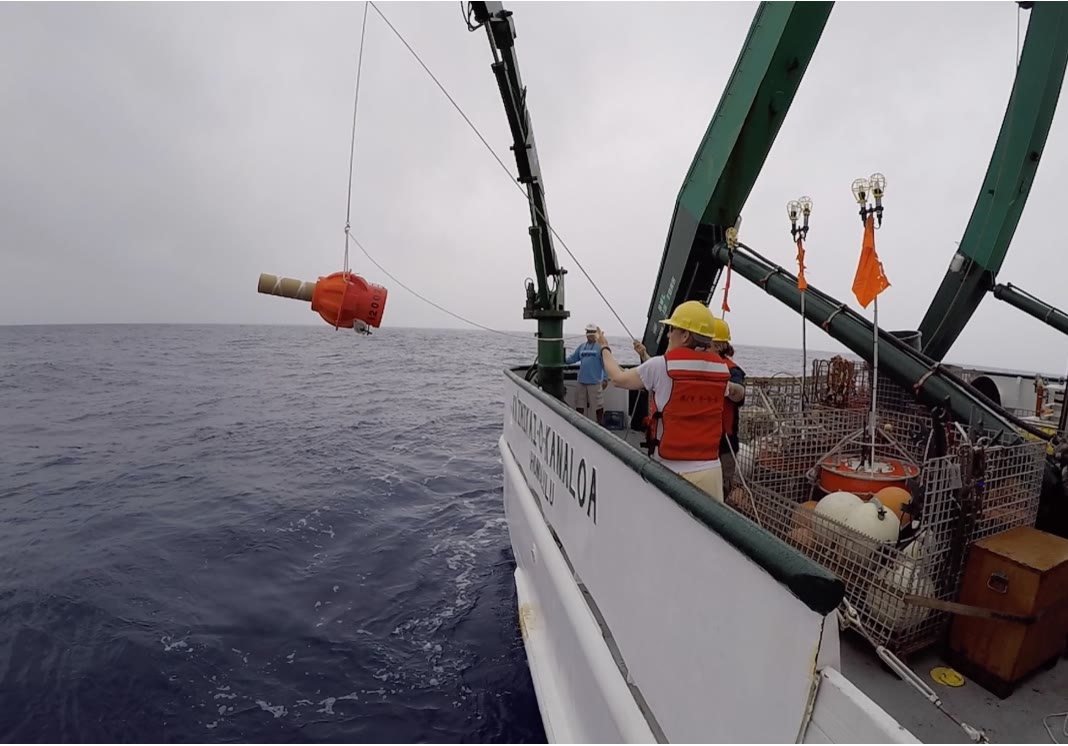
\includegraphics[width=0.6\linewidth]{images/book3/b1-deep-float.jpg}

{\small A deep-ocean profiling float (the orange instrument hanging from the crane)
being lowered from a research vessel in 2018; once released, it sinks to its
working depth and surfaces at regular intervals to send its data. (Unidentified NOAA
photographer, public domain, via Wikimedia Commons.)}
\label{fig:b1:ocean-circulation:float}
\end{omfigure}
% ledger: commons:deep-solo, noaa:argo-25

The overturning carries heat. Water that goes north warm and comes back cold has
given up heat to the atmosphere of the north.

\begin{proposition}[Heat carried by an overturning]\label{prop:b1:ocean-circulation:heat}
If a volume transport $Q$ crosses a \omterm{def:b1:spherical-astronomy:geographic}{latitude} northward at the \omterm{def:b1:fluid-envelopes-structure:potential-temperature}{potential temperature}
$\theta_1$ and returns southward at $\theta_2$, with no net transport of mass, the
overturning carries northward the heat flux
\[
  H = \rho c_p\,Q\,(\theta_1 - \theta_2),
\]
where $c_p$ is the specific heat of seawater.
\end{proposition}
% ledger: teos10:cp0

\begin{proof}
Each second, the mass $\rho Q$ crosses northward carrying the heat content $\rho Q
c_p\theta_1$, counted from an arbitrary zero of temperature, and the same mass
crosses southward carrying $\rho Q c_p\theta_2$. The net northward flux is the
difference; because the two masses are equal, the arbitrary zero cancels, and the
result is a true transport of heat.
\end{proof}

A rough budget of the North Atlantic, by W.~Schmitz, has the Gulf Stream carrying
\qty{40}{\sverdrup} of water at \qty{18}{\celsius} north, of which
\qty{14}{\sverdrup} return south as deep water at \qty{2}{\celsius}. With $c_p =
\qty{3992}{J.kg^{-1}.K^{-1}}$ and $\rho = \qty{1027}{kg.m^{-3}}$, this overturning
carries $1027 \times 3992 \times \num{14e6} \times 16 = \qty{0.92e15}{W}$, about
\qty{0.9}{PW}, north of \ang{24} N; careful estimates give \qty{1.2}{PW}, a
quarter of the poleward transport of heat by the atmosphere and the ocean
combined. Most of this heat is given to the air over the northern North
Atlantic, which is one reason why Norway, at \ang{60} N, is far warmer than southern
Greenland at the same \omterm{def:b1:spherical-astronomy:geographic}{latitude}.
% ledger: stewart:heat-conveyor, rapid:home, teos10:cp0 (computed in calc/ch29.py)

The deep circulation is slow. If it takes about a thousand years for water sinking
in the North Atlantic to reach the North Pacific by way of the Antarctic Circumpolar
Current, its mean speed is about \qty{1}{mm/s}, a hundred times less than the
variable deep currents that a current meter records. Its speed is therefore inferred
from tracers rather than measured: tritium, released into the atmosphere by the
nuclear tests of the 1950s and decaying with a half-life of 12.3 years, entered the
deep North Atlantic where deep water forms, and after 25 years had spread little
south of \ang{30} N, a mean speed of less than \qty{1}{mm/s}. The volume of the ocean
divided by the rate at which deep water forms gives the same order of time
(\cref{exo:b1:ocean-circulation:12}).
% ledger: stewart:deep-circulation, nos:conveyor

The Antarctic Circumpolar Current joins the basins. Its currents reach the sea floor
and are slow, about \qty{10}{cm/s}, up to \qty{50}{cm/s} at its fronts, but it is
deep and wide: an array of moored current meters across Drake Passage,
between South America and Antarctica, gave \qty[uncertainty-mode=separate]{125 \pm
11}{\sverdrup} (published in 1985), and a denser array in 2007--2011,
which measured the currents near the bottom as well, gave \qty{173.3}{\sverdrup},
\qty{30}{\percent} more than that long-used value. It carries deep water from each
ocean to the others and mixes it on the way.
% ledger: stewart:acc, donohue:acc

\begin{dated}{2021}
% ledger: ipcc:amoc-observed, ipcc:amoc-projected
The 2021 assessment of the Intergovernmental Panel on Climate Change finds, from
reconstructions, that the Atlantic overturning was relatively stable over the past
\num{8000} years (\emph{medium confidence}), with a weakening beginning in the late
19th century (\emph{medium confidence}), but has only \emph{low confidence} in an
overall decline during the 20th century. The weakening observed directly from the
mid-2000s to the mid-2010s (\emph{high confidence}) cannot be told apart from
decade-scale variability (\emph{high confidence}). The overturning is \emph{very
likely} to weaken over the 21st century for all emissions scenarios, with only
\emph{low confidence} in the size of the decline; there is \emph{medium confidence}
that it will not collapse abruptly before 2100.
\end{dated}

\section{Exercises}

\begin{exercise}[$\star$]\label{exo:b1:ocean-circulation:1}
Use the bulk formula with $\rho_a = \qty{1.3}{kg.m^{-3}}$ and the drag coefficient
of Yelland and Taylor. (a)~Compute $C_D$ and the \omterm{def:b1:ocean-circulation:wind-stress}{wind stress} for winds of 4, 7 and
\qty{15}{m/s}. (b)~By what factor does the stress grow from 7 to \qty{15}{m/s}?
Compare with the ratio of the squares of the speeds and explain the difference.
% ledger: stewart:wind-stress, stewart:drag-coefficient
\end{exercise}

\begin{exercise}[$\star$]\label{exo:b1:ocean-circulation:2}
Give the direction of the \omterm{def:b1:ocean-circulation:ekman}{Ekman transport} in each case. (a)~A wind blowing towards
the east at \ang{45} N. (b)~A trade wind from the north-east at \ang{15} N.
(c)~A wind blowing towards the east at \ang{50} S. (d)~A wind from the south along
the west coast of southern Africa, near \ang{23} S. In which of the four cases does
the transport point offshore, and what follows?
\end{exercise}

\begin{exercise}[$\star$]\label{exo:b1:ocean-circulation:3}
At \ang{26.5} N in the Atlantic, the mean transports of 2004--2024 are: Strait of
Florida \qty{31.7}{\sverdrup}, Ekman \qty{3.5}{\sverdrup}, upper mid-ocean
\qty{-17.9}{\sverdrup}; by layers, 0--\qty{800}{m} \qty{16.6}{\sverdrup},
800--\qty{1100}{m} \qty{0.4}{\sverdrup}, 1100--\qty{3000}{m} \qty{-12.0}{\sverdrup},
3000--\qty{5000}{m} \qty{-5.9}{\sverdrup} (northward positive). (a)~Add the first
three and compare with the published overturning, \qty{17.1}{\sverdrup}. (b)~Compare
the northward flow above \qty{1100}{m} with the southward flow below. (c)~Convert
\qty{17.1}{\sverdrup} into cubic kilometres per year, and compute the time this flow
would take to fill the volume of the whole ocean, \qty{1.3324e9}{km^3}.
% ledger: rapid:transports, charette:ocean-volume
\end{exercise}

\begin{exercise}[$\star$]\label{exo:b1:ocean-circulation:4}
With Ekman's formulas, compute the Ekman depth and the surface current under a wind
of \qty{10}{m/s} at \ang{15}, \ang{45} and \ang{60} of \omterm{def:b1:spherical-astronomy:geographic}{latitude}, and the surface
current as a percentage of the wind. Why do the formulas fail near the equator?
% ledger: stewart:ekman-constants
\end{exercise}

\begin{exercise}[$\star\star$]\label{exo:b1:ocean-circulation:5}
Across \ang{11} N in the Atlantic, take a mean \omterm{def:b1:ocean-circulation:wind-stress}{wind stress} of \qty{0.07}{Pa} towards
the west over a width of \qty{5000}{km}, and $\rho = \qty{1027}{kg.m^{-3}}$.
(a)~Compute the \omterm{def:b1:ocean-circulation:ekman}{Ekman transport} per metre and its direction. (b)~Compute the total
volume transport across the section in \omterm{def:b1:ocean-circulation:ekman}{sverdrups}. (c)~Compare with the transports
measured directly ($12.0 \pm \qty{5.5}{\sverdrup}$) and computed from long-term
winds ($13.5 \pm \qty{0.3}{\sverdrup}$).
% ledger: stewart:ekman-transport
\end{exercise}

\begin{exercise}[$\star\star$]\label{exo:b1:ocean-circulation:6}
Along the equatorial Pacific, the \omterm{def:b1:atmospheric-circulation:winds}{trade winds} exert a stress of \qty{0.05}{Pa}
towards the west. (a)~Compute the \omterm{def:b1:ocean-circulation:ekman}{Ekman transport} per metre, and its direction, at
\ang{2} N and at \ang{2}~S. (b)~Assuming that the water carried away across these two
\omterm{def:b1:spherical-astronomy:geographic}{latitudes} is replaced from below between them, compute the mean \omterm{def:b1:ocean-circulation:upwelling}{upwelling} velocity
in metres per day. (c)~What happens to the formula of the theorem at the equator
itself? Which conclusion survives?
\end{exercise}

\begin{exercise}[$\star\star$]\label{exo:b1:ocean-circulation:7}
Over a \omterm{def:b1:ocean-circulation:gyre}{subtropical gyre}, take a \omterm{def:b1:ocean-circulation:wind-stress}{wind stress} of \qty{0.06}{Pa} towards the west at
\ang{15} N and \qty{0.12}{Pa} towards the east at \ang{40} N. (a)~Compute both \omterm{def:b1:ocean-circulation:ekman}{Ekman
transports} and their directions. (b)~Assuming the transport changes uniformly between
the two \omterm{def:b1:spherical-astronomy:geographic}{latitudes}, compute the vertical velocity at the base of the \omterm{def:b1:ocean-circulation:ekman}{Ekman layer}, in
metres per year, and say whether it is upward or downward. (c)~Over a basin
\qty{5000}{km} wide, how many \omterm{def:b1:ocean-circulation:ekman}{sverdrups} are pumped through the base of the layer?
\end{exercise}

\begin{exercise}[$\star\star$]\label{exo:b1:ocean-circulation:8}
Take $\rho = \qty{1027}{kg.m^{-3}}$ and $c_p = \qty{3992}{J.kg^{-1}.K^{-1}}$.
(a)~Compute the heat carried north by \qty{17}{\sverdrup} flowing north at
\qty{15}{\celsius} and returning at \qty{3}{\celsius}. (b)~Compare with the
\qty{1.2}{PW} carried by the Atlantic overturning. (c)~If the same water returned
south at the surface, along the eastern side of the basin, at \qty{12}{\celsius},
what heat would it carry? What does this say about the importance of \omterm{def:b1:ocean-circulation:moc}{deep-water
formation}?
% ledger: rapid:home, teos10:cp0
\end{exercise}

\begin{exercise}[$\star\star$]\label{exo:b1:ocean-circulation:9}
Three water masses of the South Atlantic have the \omterm{def:b1:fluid-envelopes-structure:potential-temperature}{potential temperatures} and
salinities: Antarctic Intermediate Water \qty{3.3}{\celsius}, 34.15; North Atlantic
Deep Water \qty{4.0}{\celsius}, 35.00; Antarctic Bottom Water \qty{0.4}{\celsius},
34.67. A sample at depth has $\theta = \qty{2.78}{\celsius}$ and $S = 34.731$.
Using \cref{prop:b1:fluid-envelopes-structure:mixing}, find the fraction of each
\omterm{def:b1:fluid-envelopes-structure:ts-diagram}{water mass} in the sample.
% ledger: stewart:deep-circulation
\end{exercise}

\begin{exercise}[$\star\star\star$]\label{exo:b1:ocean-circulation:10}
Take the spiral of \cref{prop:b1:ocean-circulation:spiral}. (a)~Show that $u$ and $v$
satisfy $f v + A_z u'' = 0$ and $-f u + A_z v'' = 0$. (Hint: write $u + iv =
V_0\,e^{i\pi/4}\,e^{(1+i)az}$.) (b)~Show that the stress $\rho A_z\,\partial\vec
v/\partial z$ at the surface equals the \omterm{def:b1:ocean-circulation:wind-stress}{wind stress} $(0, T)$. (c)~Compute the
transports $\int_{-\infty}^0 \rho u\,\mathrm dz$ and $\int_{-\infty}^0 \rho
v\,\mathrm dz$, and check that they agree with
\cref{thm:b1:ocean-circulation:ekman}.
\end{exercise}

\begin{exercise}[$\star\star\star$]\label{exo:b1:ocean-circulation:11}
In Stommel's model, the \omterm{def:b1:ocean-circulation:wbc}{western boundary current} has a width of about $R/\beta$,
where $R$ is the rate of bottom friction and $\beta = \mathrm df/\mathrm dy$ the
northward rate of increase of the \omterm{def:b1:atmospheric-circulation:coriolis-parameter}{Coriolis parameter}. (a)~Show that $\beta = 2\Omega
\cos\varphi/a_\oplus$ and compute it at \ang{30} N ($a_\oplus = \qty{6371}{km}$).
(b)~With $R = \qty{e-6}{s^{-1}}$, compute the width. (c)~A transport of
\qty{30}{\sverdrup} drifts south across the interior of a basin \qty{5000}{km} wide
in the upper \qty{1000}{m}, and returns north in the boundary current over the same
depth. Compute both mean speeds and compare with the speed of the Gulf Stream,
\qty{1.8}{m/s}.
% ledger: stewart:north-atlantic, nos:gulf-stream, earth:Rmean
\end{exercise}

\begin{exercise}[$\star\star\star$]\label{exo:b1:ocean-circulation:12}
The ocean holds \qty{1.3324e9}{km^3} over \qty{361.84e6}{km^2}. (a)~Show that the
volume below \qty{1000}{m} is at least \qty{9.71e8}{km^3}. (b)~North Atlantic Deep
Water forms at about \qty{17}{\sverdrup} and Antarctic Bottom Water at about
\qty{9}{\sverdrup}. Estimate the time needed to renew the water below
\qty{1000}{m}, and compare with the thousand years of the conveyor. (c)~Tritium has a
half-life of 12.3 years. What fraction of a tritium input remains after 25 years? How
far does water moving at \qty{1}{mm/s} travel in 25 years?
% ledger: charette:ocean-volume, stewart:deep-circulation, stewart:acc, rapid:transports
\end{exercise}

\section{Problem: An upwelling coast}

\begin{problem}[{Weekend problem --- a summer wind along a coast at \ang{38} N}]
\label{pb:b1:ocean-circulation:1}
% values: calc/ch29.py (invented coast; constants from the ledger)
A straight coast runs north--south at \ang{38} N, with the ocean to the west. In
summer, a steady wind of \qty{8}{m/s} blows from the north along it for weeks. The
coast is invented, but its numbers are typical of the eastern sides of the oceans.
Use $\Omega = 2\pi/(\qty{23.9345}{h})$, $\rho_a = \qty{1.3}{kg.m^{-3}}$, the drag
coefficient of Yelland and Taylor, $\rho = \qty{1027}{kg.m^{-3}}$ for seawater and
$c_p = \qty{3992}{J.kg^{-1}.K^{-1}}$.

\medskip
\noindent\textbf{Part I --- The wind and its stress.}
\begin{enumerate}
  \item Towards which direction does the wind blow? Is it along the coast or across
        it?
  \item Compute the drag coefficient.
  \item Compute the \omterm{def:b1:ocean-circulation:wind-stress}{wind stress}.
  \item Same two questions for a wind of \qty{12}{m/s}. By what factor does the
        stress grow, and why is it more than the ratio of the squares of the speeds?
  \item Compute the \omterm{def:b1:atmospheric-circulation:coriolis-parameter}{Coriolis parameter} at \ang{38} N.
  \item Compute $2\pi/f$ in hours. Why must the wind blow for a day or more before
        the Ekman balance applies?
\end{enumerate}

\medskip
\noindent\textbf{Part II --- The Ekman layer.}
\begin{enumerate}[resume]
  \item In which direction is the \omterm{def:b1:ocean-circulation:ekman}{Ekman transport}? Towards the land or the open sea?
  \item Compute the Ekman mass transport per metre of coast.
  \item Convert it into a volume transport per metre.
  \item Compute the Ekman depth with Ekman's formula.
  \item Compute the mean offshore velocity in the layer, in \unit{cm/s}.
  \item Compute the surface current with Ekman's formula, and its direction. What
        do the drifter measurements suggest instead for its speed?
\end{enumerate}

\medskip
\noindent\textbf{Part III --- Upwelling at the coast.}
\begin{enumerate}[resume]
  \item Explain, with a sketch of a vertical section, where the water carried
        offshore comes from.
  \item Compute the volume upwelled per day along each kilometre of coast.
  \item Suppose the water rises through a band \qty{20}{km} wide along the coast.
        Compute the mean upward velocity, in \unit{m/s} and in metres per day.
  \item How long does water take to rise from the base of the \omterm{def:b1:ocean-circulation:ekman}{Ekman layer} to the
        surface at this speed?
  \item The upwelled water reaches the surface at \qty{12}{\celsius}, while the
        open sea offshore is at \qty{18}{\celsius}. The sea breeze carries warm,
        moist air from offshore over this water. What happens to the air near the
        surface, and what weather follows on the coast?
  \item Why are such coasts rich in fish?
  \item In autumn the wind turns and blows from the south for a week. What happens
        to the transport and to the water at the coast?
\end{enumerate}

\medskip
\noindent\textbf{Part IV --- Other coasts and the total transport.}
\begin{enumerate}[resume]
  \item With the same stress, compute the \omterm{def:b1:ocean-circulation:ekman}{Ekman transport} per metre at \ang{20} N
        and compare with \ang{38} N.
  \item On the west coast of southern Africa, near \ang{23} S, which wind direction
        drives \omterm{def:b1:ocean-circulation:upwelling}{upwelling}? Compare with the coast of the problem.
  \item Under a wind of \qty{5}{m/s} instead of \qty{8}{m/s} at \ang{38} N, compute
        the stress and the \omterm{def:b1:ocean-circulation:ekman}{Ekman transport} per metre, and their ratio to those of
        question~8.
  \item The upwelled water warms by \qty{6}{\celsius} as it drifts offshore. Compute
        the heat it takes up per second per metre of coast, then along
        \qty{1000}{km}.
  \item What length of such a coast would upwell as much water as the Gulf Stream
        carries through the Strait of Florida, \qty{31.7}{\sverdrup}?
  \item What volume of water, in \omterm{def:b1:ocean-circulation:ekman}{sverdrups}, is upwelled along \qty{1000}{km} of this
        coast?
\end{enumerate}
\end{problem}
